\chapter{Background}
\label{ch:background}

\section{Sample stuff}
Some simple and useful latex formatting.

\subsection{Quotations and citing}
It is explained in detail in \cite[Ch.20]{Norvig03} that 
\begin{quotation}
\noindent \textit{``the true hypothesis eventually dominates the Bayesian predication. For any fixed prior that does not rule out the true hypothesis, the posterior probability of any false hypothesis will eventually vanish, simply because the probability of generating ``uncharacteristic'' data indefinitely is vanishingly small.''}
\end{quotation}
\subsection{Figures}
This distribution, and its probability density function, is displayed in Figure \ref{fig:gaussian_distr_pdf}.
\begin{figure}[ht]
	\center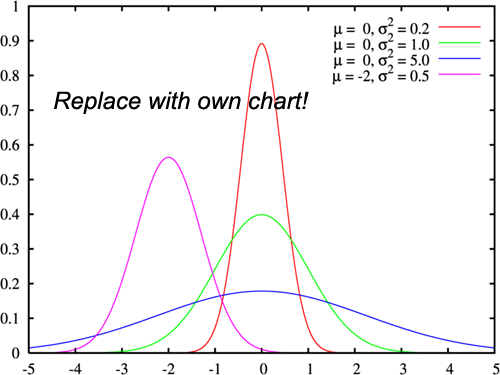
\includegraphics[width=10cm]{images/normal_distr_pdf}	
	\label{fig:gaussian_distr_pdf}
	\caption{The Normal distribution PDF.}
\end{figure}

\subsection{Equations}
By using these probabilities, and Bayes formula, we can derive the Bayes classifier.
\begin{equation}
	P(\omega_i | \boldsymbol{x}, \mathcal{X}) = \frac{p(\boldsymbol{x}|\omega_i, \mathcal(X))P(\omega_i|\mathcal{X})}{\sum_{j=1}^{c}p(\boldsymbol{x}|\omega_j, \mathcal{X})P(\omega_j|\mathcal{X})},
	\label{eq:bayes_formula_1}
\end{equation}
when we can separate the training samples by class into $c$ subsets $\mathcal{X}_1, \ldots, \mathcal{X}_c$, with the samples in $\mathcal{X}_i$ belonging to $\omega_i$.

